\section{Implementierung}

\subsection{Quantenalgorithmus}
Wie im Kapitel~\ref*{Funktionsweise} zur Funktionsweise erklärt,
wird für die Periodenbestimmung die Quanten-Phase-Estimation genutzt.

Um den Quanten-Phase-Estimation Algorithmus für die Periodenberechnung zu nutzen,
benötigt man ein Gatter \(U\) welches die modulare Multiplikation \(U\ket{y} = \ket{ay \mod N}\), 
als eine unitär Transformation realisiert.
Mit den passenden \(U\)-Gatter wird der Quantenschaltkreis wie in Abbildung~\ref{fig:shor_n_qubit} strukturiert.
\begin{figure}
    \caption{QPE für Shor~\cite{anonymousket}}
    \label{fig:shor_n_qubit}
    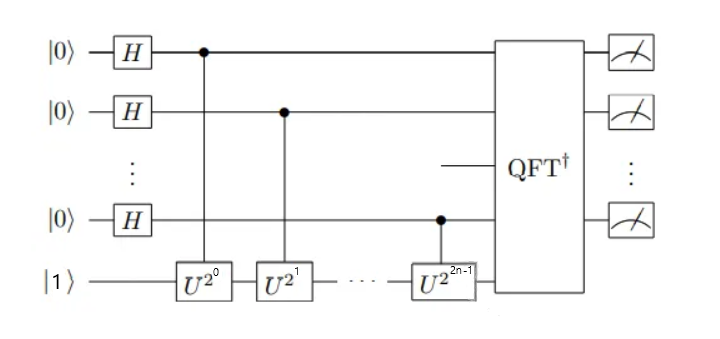
\includegraphics[width=\columnwidth]{shor_n_qubit.png}
    \centering
    \end{figure}

Die Realisierung der Transformation bedingt die Implementierung einiger arithmetischer Operationen in Form eines Quantenschaltkreises. 
Diese fungieren als Bausteine, die zusammengesetzt zur Konstruktion des übergeordneten Quantenschaltkreises für die modulare Multiplikation beitragen. 
Zu den erforderlichen arithmetischen Operationen gehört die Addition, Subtraktion sowie die modulare Addition.

In den folgenden Abschnitten werden die untergeordneten arithmetischen Operationen bis hin zur modularen Multiplikation implementiert.

\subsubsection{Addition}
Der Quantenschaltkreis für die Addition bildet das Fundament der \(U\)-Gatter und 
stellt einen der am häufigsten verwendeten Bausteine dar. 
Deswegen hat die Implementierung der Addition einen erheblichen Einfluss auf den Ressourcenbedarf des gesamten Quantenalgorithmus
und sollte daher möglichst effizient implementiert werden.

Eine Möglichkeit, die Addition als Quantenschaltkreis zu realisieren, 
besteht im Nachbau eines klassischen Schaltkreises aus Volladdierern. 
Da es nicht möglich ist, 
die notwendige klassischen Gatter wie AND und OR als unitäre Transformation mit nur zwei Qubits darzustellen~\cite{Hoever2023QC},
werden zusätzliche Hilfsqubits benötigt.
Die zusätzlichen Hilfsqubits bewirken, dass der Nachbau eines klassischen Schaltkreis für die Addition zweier \(n\)-Bit Zahlen, 
also solche der Größenordnung \(2^n\), mindestens \(3n\) Qubits benötigt~\cite{zalka1998fast}.

Eine effizientere Methode, die ohne Hilfsqubits auskommt, ist die Quanten-Addition~\cite{draper2000addition}. 
Die Quanten-Addition führt die Berechnung auf quantenmechanische Weise durch. 
Im Wesentlichen wird dabei die Addition in der Fourier-Basis berechnet, 
wobei die Phasen der Qubits eines Summanden mit kontrollierte Phasenverschiebungen auf die Qubits des anderen Summanden wirkt.

Im Folgenden wird ein Beispiel für die Quanten-Addition zweier Qubit-Register \(\ket{a}_3\) und \(\ket{b}_3\), 
jeweils bestehend aus drei Qubits, betrachtet:
\begin{figure}[H]
    \caption{Quantum-Addition}
    \label{fig:3_qubit_quantum_add}
    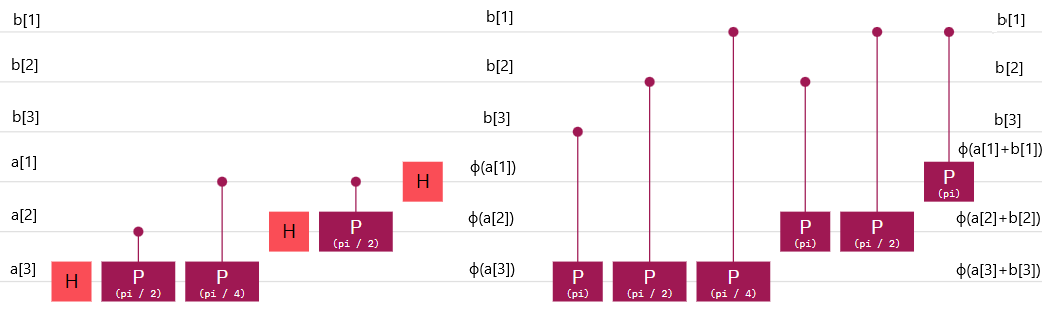
\includegraphics[width=\columnwidth]{3_qubit_quantum_add.png}
    \centering
    \end{figure}
Die Registermarkierungen in der Mitte von Abbildung~\ref*{fig:3_qubit_quantum_add} unterteilen die Darstellung in zwei Hälften.
Die linke Hälfte repräsentiert die Quanten-Fourier-Transformation, 
während die rechte Hälfte die Quanten-Addition zeigt.

Wie man an der Struktur der Quanten-Addition erkennen kann,
ist die Anordnung der Gatter fast identisch mit der Quanten-Fourier-Transformation.
Ein Unterschied besteht darin, 
dass die Hadamard-Gatter durch kontrollierte \(P(\pi)\) Phasen-Gatter ersetzt wurden.
Sowohl das Hadamard-Gatter als auch das \(P(\pi)\) Phasen-Gatter erzeugen eine relative Phase von \(e^{\pi i}\).
Ein weiterer Unterschied zur Quanten-Fourier-Transformation besteht darin, 
dass die Phasen-Gatter nicht durch das gleiche Register\(\ket{a}_3\) kontrolliert werden, 
auf das die Gatter auch wirken.
Stattdessen kontrollieren die Qubits des Registers \(\ket{b}_3\) die Phasen-Gatter.
Dabei wird das \(P(\pi)\) Phasen-Gatter durch das Qubit des \(\ket{b}_3\) kontrolliert,
welches die selbe Wertigkeit hat wie das Zielqubit des \(\ket{a}_3\) Registers.
Jedes weitere kontrollierte Phasen-Gatter für das gleiche Zielqubit 
wird fortlaufend von dem nächstkleineren Qubit von \(\ket{b}_3\) kontrolliert.

Im Prinzip handelt es sich bei dieser Quantenschaltung um eine Anwendung derselben Phasenverschiebungen 
wie bei der Quanten-Fourier-Transformation. 
Der grundlegende Unterschied liegt darin, 
dass diese Phasenverschiebungen kontrolliert auf ein anderes Quantenregister angewendet werden.

Die Wirkung der Quanten-Addition wird anhand der Abbildung~\ref*{fig:3_qubit_quantum_add} verdeutlicht:
Am Anfang der linken Hälfte befinden sich beide Register in der Standardbasis.
Auf das Zielregister \(\ket{a}_3\) wirkt die Quanten-Fourier-Transformation ohne Swap Gatter.
Dadurch befindet sich \(\ket{a}_3\) nun in der Fourier-Basis \(\Phi\), also \(\ket{\Phi(a)}_3\):
\[\ket{\Phi(a)}_3 = \frac{1}{\sqrt{8}} [ (\ket{0} + { e^{\frac{2 \pi i (2^0a_1)}{2^1}}}\ket{1} ) \bigotimes
( \ket{0} + { e^{\frac{2 \pi i (2^1a_2+2^0a_1)}{2^2}}}\ket{1} ) \bigotimes
( \ket{0} + { e^{\frac{2 \pi i (2^{2}a_3 +2^1a_2+2^0a_1)}{2^3}}}\ket{1} ) ] \]
Anschließend wirkt auf das hinterste Tensorprodukt ein \(P(\pi)\) Phasen-Gatter,
welches durch \(\ket{b_3}_1\) kontrolliert wird.
Wenn sich \(\ket{b_3}_1\) im Zustand \(\ket{0}_1\) befindet, passiert nichts.
Wenn es sich im Zustand \(\ket{1}_1\) befindet, dass das Phasen-Gatter angewendet wird.
Dieses Verhalten kann man für beide Fälle mit den entsprechenden Matrizen 
\(\begin{pmatrix}
    1 & 0 \\
    0 & e^{\pi i b_3}
  \end{pmatrix}\)
  beziehungsweise  
  \(\begin{pmatrix}
    1 & 0 \\
    0 & e^{\frac{2\pi i (2^2b_3)}{2^3}}
  \end{pmatrix}\)
beschreiben.
Schreibt man das hinterste Tensorprodukt als Vektor, ergibt sich die folgende Formulierung:
\[\frac{1}{\sqrt{2}}( \ket{0} + { e^{\frac{2 \pi i (2^{2}a_3 +2^1a_2+2^0a_1)}{2^3}}}\ket{1}) \equiv
\frac{1}{\sqrt{2}}
\begin{pmatrix}
     1  \\
     e^{\frac{2 \pi i (2^{2}a_3 +2^1a_2+2^0a_1)}{2^3}}
  \end{pmatrix}
    \]
Dann wird durch das Ergebnis der Verrechnung mit dem Phasen-Gatter deutlich, 
dass die Addition im Wesentlichen in der Phase des Quantenzustands stattfindet:
\[\begin{pmatrix}
    1 & 0 \\
    0 & e^{\frac{2\pi i (2^2b_3)}{2^3}}
  \end{pmatrix}
    \cdot
\frac{1}{\sqrt{2}}
\begin{pmatrix}
    1  \\
     e^{\frac{2 \pi i (2^{2}a_3 +2^1a_2+2^0a_1)}{2^3}}
  \end{pmatrix}
  =
  \frac{1}{\sqrt{2}}
  \begin{pmatrix}
    1  \\
     e^{\frac{2 \pi i (2^{2}(a_3+b_3) +2^1a_2+2^0a_1)}{2^3}}
  \end{pmatrix}
\]
Wie in der Abbildung~\ref*{fig:3_qubit_quantum_add} erkenntlich,
wirken auf das hinterste Tensorprodukt auch noch die beiden Phasen-Gatter \(P(\frac{\pi}{2})\) und \(P(\frac{\pi}{4})\) mit:
\[
    P(\frac{\pi}{2}) = 
\begin{pmatrix}
    1 & 0 \\
    0 & e^{\frac{\pi}{2} i b_2}
  \end{pmatrix}
  =
  \begin{pmatrix}
    1 & 0 \\
    0 & e^{\frac{2\pi i (2^1b_2)}{2^3}}
  \end{pmatrix}
  ~;~
P(\frac{\pi}{4}) = 
\begin{pmatrix}
    1 & 0 \\
    0 & e^{\frac{\pi}{4} i b_1}
  \end{pmatrix}
  =
  \begin{pmatrix}
    1 & 0 \\
    0 & e^{\frac{2\pi i (2^0b_1)}{2^3}}
  \end{pmatrix}
\]
\[
    \begin{pmatrix}
        1 & 0 \\
        0 & e^{\frac{2\pi i (2^0b_1)}{2^3}}
      \end{pmatrix}
      \cdot
      \begin{pmatrix}
        1 & 0 \\
        0 & e^{\frac{2\pi i (2^1b_2)}{2^3}}
      \end{pmatrix}
      \cdot
      \frac{1}{\sqrt{2}}
      \begin{pmatrix}
        1  \\
         e^{\frac{2 \pi i (2^{2}(a_3+b_3) +2^1a_2+2^0a_1)}{2^3}}
      \end{pmatrix}
      =
      \frac{1}{\sqrt{2}}
      \begin{pmatrix}
        1  \\
         e^{\frac{2 \pi i (2^{2}(a_3+b_3) +2^1(a_2+b_2)+2^0(a_1+b_1))}{2^3}}
      \end{pmatrix}
\]
Wendet man alle weiteren Phasen-Gatter auf das vollstände Tensorprodukt an, 
erhält man:
\[
    \frac{1}{\sqrt{8}} [ (\ket{0} + { e^{\frac{2 \pi i (2^0(a_1+b_1))}{2^1}}}\ket{1} ) \bigotimes
( \ket{0} + { e^{\frac{2 \pi i (2^1(a_2+b_2)+2^0(a_1+b_1))}{2^2}}}\ket{1} ) \bigotimes
( \ket{0} + { e^{\frac{2 \pi i (2^{2}(a_3+b_3) +2^1(a_2+b_2)+2^0(a_1+b_1))}{2^3}}}\ket{1} ) ]
\]
Setzt man in diese Formel zwei Zahlen in Binärschreibweise ein, 
wird man den selben Zustand erhalten,
wie wenn man die Summe der beiden Zahlen in die Formel der Quanten-Fourier-Transformation einsetzt.
Beispielsweise sei \(a = 3\) also binär \(a_3 = 0\), \(a_2 = 1\),\(a_1 = 1\) und 
\(b = 1\) also \(b_3 = 0\), \(b_2 = 0\),\(b_1 = 1\):
\[
\frac{1}{\sqrt{8}} [ (\ket{0} + { e^{\frac{2 \pi i (2^0(1+1))}{2^1}}}\ket{1} ) \bigotimes
( \ket{0} + { e^{\frac{2 \pi i (2^1(1+0)+2^0(1+1))}{2^2}}}\ket{1} ) \bigotimes
( \ket{0} + { e^{\frac{2 \pi i (2^{2}(0+0) +2^1(1+0)+2^0(1+1))}{2^3}}}\ket{1} ) ]
\]
\[
=\frac{1}{\sqrt{8}} [ (\ket{0} + \ket{1} ) \bigotimes
( \ket{0} +   \ket{1} ) \bigotimes
( \ket{0} +  e^{\pi i }\ket{1} ) ]
\]
Das dies tatsächlich die Summe in Fourier-Basis entspricht, 
wird deutlich wenn man das selbe Tensorprodukt aus der Quanten-Fourier-Transformation bildet:
\[
    QFT(\ket{c}_3)
    \frac{1}{\sqrt{8}} [ (\ket{0} + { e^{\frac{2 \pi i (2^0(c_1))}{2^1}}}\ket{1} ) \bigotimes
( \ket{0} + { e^{\frac{2 \pi i (2^1(c_2)+2^0(c_1))}{2^2}}}\ket{1} ) \bigotimes
( \ket{0} + { e^{\frac{2 \pi i (2^{2}(c_3) +2^1(c_2)+2^0(c_1))}{2^3}}}\ket{1} ) ]
\]
Die Summe von \(a\) und \(b\) entspricht \(c = 4\) also \(c_3 = 1,~c_2 = 0,~c_1=0\):
\[
    QFT(\ket{4}_3)
    \frac{1}{\sqrt{8}} [ (\ket{0} + { e^{\frac{2 \pi i (2^0(0))}{2^1}}}\ket{1} ) \bigotimes
( \ket{0} + { e^{\frac{2 \pi i (2^1(0)+2^0(0))}{2^2}}}\ket{1} ) \bigotimes
( \ket{0} + { e^{\frac{2 \pi i (2^{2}(1) +2^1(0)+2^0(0))}{2^3}}}\ket{1} ) ]
\]
\[
    = 
    \frac{1}{\sqrt{8}} [ (\ket{0} + { e^{\frac{2 \pi i (0)}{2^1}}}\ket{1} ) \bigotimes
( \ket{0} + { e^{\frac{2 \pi i (0)}{2^2}}}\ket{1} ) \bigotimes
( \ket{0} + { e^{\frac{2 \pi i (2^{2}(1))}{2^3}}}\ket{1} ) ]
\]
\[
=\frac{1}{\sqrt{8}} [ (\ket{0} + \ket{1} ) \bigotimes
( \ket{0} +   \ket{1} ) \bigotimes
( \ket{0} +  e^{\pi i }\ket{1} ) ]
\]
Das Ergebnis der Quanten-Addition zweier Summanden \(a=3,~b=1\), 
jeweils in einem Register mit drei Qubits,
ist somit identisch mit dem Zustand, 
der durch die Anwendung der Quanten-Fourier-Transformation auf ein Register 
aus ebenfalls drei Qubits mit der Summe der beiden Zahlen entsteht.

Mit einer anschließenden inversen Quanten-Fourier-Transformation, 
kann die Summe in die Standardbasis und somit in einen Messbaren Zustand transformiert werden:
\[
iQFT(\ket{\Phi(4)_3})
\equiv
 iQFT(\frac{1}{\sqrt{8}} [ (\ket{0} + \ket{1} ) \bigotimes
( \ket{0} +   \ket{1} ) \bigotimes
( \ket{0} +  e^{\pi i }\ket{1} ) ]) 
=
\ket{4}_3
\]

Das Zielregister sollte aus genügend Qubits bestehen, 
damit die Summe vollständig erfasst werden kann.
Andernfalls kommt es zum overflow mit \(a + b \mod 2^n\), 
wobei \(n\) die Anzahl an Qubits des Zielregisters beschreibt~\cite{beauregard2003circuit}.

Für die Realisierung der modularen Multiplikation wird zu keinem Zeitpunkt der Berechnung eine Addition zweier Zwischenergebnisse benötigt. 
Genauer gesagt, ist es nicht nötig, ein Quantenregister auf ein anderes zu addieren. 
Stattdessen wird die Quanten-Addition benutzt, um eine vorab bekannte Zahl auf ein Quantenregister zu addieren.

Bei der Quanten-Addition mit zwei Register wie in Abbildung~\ref{fig:3_qubit_quantum_add} erfolgt die Phasenverschiebung kontrolliert,  
also in Abhängigkeit des Inhaltes von Register \(\ket{b}_3\).
Ist der Inhalt von Register \(\ket{b}_3\) vorab bekannt,
können gewöhnliche Phasen-Gatter anstelle von kontrollierten verwendet werden~\cite{beauregard2003circuit}.

Wenn bei der Quanten-Addition mit zwei Registern ein Phasen-Gatter aufgrund des zugehörigen Kontrollqubits im Zustand \(\ket{1}\) angewendet wird,
wird es in der Variante mit einem einzelnen Register als gewöhnliches Phasen-Gatter verwendet.
Ist das Kontrollqubit hingegen im Zustand \(\ket{0}\), 
wodurch das Phasen-Gatter bei der Quanten-Addition mit zwei Registern nicht zur Anwendung kommt, 
wird dieses Phasen-Gatter in der Variante mit nur einem Register weggelassen.

\begin{figure}[H]
    \caption{Quantum-Addition fixierte Phasenverschiebungen}
    \label{fig:3_qubit_fixed_quantum_addition}
    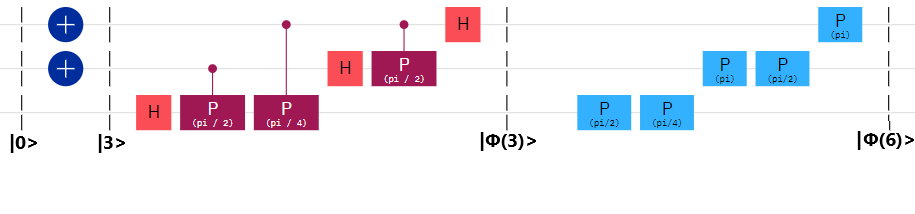
\includegraphics[width=\columnwidth]{3_qubit_fixed_quantum_addition.png}
    \centering
    \end{figure}
In Abbildung~\ref{fig:3_qubit_fixed_quantum_addition} ist die Quanten-Addition für ein 3-Qubit Register abgebildet.
Die blauen Phasen-Gatter sorgen für die Quanten-Addition mit einem fixierten Wert von \(3\).
Vergleicht man die Abbildung~\ref{fig:3_qubit_fixed_quantum_addition} mit der Abbildung~\ref{fig:3_qubit_quantum_add} fällt auf, 
dass das aller erste Phasen-Gatter der Quanten-Addition nicht vorkommt.
Im Quantenschaltkreis der Abbildung~\ref{fig:3_qubit_quantum_add} würde ein Registerinhalt von \(b = 3\) das Kontrollqubit \(b_3\) nicht setzen. 
Somit kommt das erste Phasen-Gatter der Quanten-Addition nicht zum Einsatz und 
wird deswegen in der Variante wie in Abbildung~\ref{fig:3_qubit_fixed_quantum_addition} weggelassen. 

Des weiteren ist es möglich, 
den Quantenschaltkreis der Quanten-Addition für eine vorab festgelegte Zahl ressourcensparender zu realisieren.
Die Optimierung bezieht sich dabei auf die Anzahl der verwendeten Gatter.
Wird die Quanten-Addition für eine feste Zahl realisiert, 
können für jedes einzelne Qubit die angewendeten Phasenverschiebungen vorab zusammengerechnet werden.
Demnach bietet es sich an, 
die zusammengerechneten Phasenverschiebung in ein einzelnes Phasen-Gatter zusammen zu fassen.
Nach diesem Prinzip, benötigt man für eine Quanten-Addition maximal ein einzelnes Phasen-Gatter pro Qubit.

\begin{figure}[H]
  \caption{Ressourcensparende Quantum-Addition}
  \label{fig:3_qubit_fixed_quantum_addition_opt}
  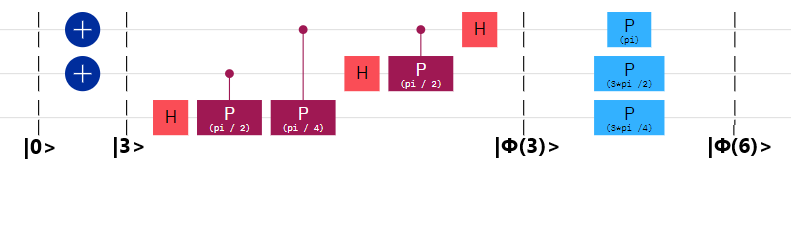
\includegraphics[width=\columnwidth]{3_qubit_fixed_quantum_addition_opt.png}
  \centering
  \end{figure}
Der Quantenschaltkreis in Abbildung~\ref{fig:3_qubit_fixed_quantum_addition_opt} führt die identische 
Berechnung durch, wie der Quantenschaltkreis aus Abbildung~\ref{fig:3_qubit_fixed_quantum_addition}.
Darüber hinaus, werden die benötigten Phasenverschiebungen mit einem einzigen Phasen-Gatter pro Qubit realisiert.

Die Implementierung nutzt die ressourceneffiziente Variante der Quanten-Addition.
In der Funktion \texttt{A\_Gate} wird ein Gatter erzeugt, 
das sämtliche für die Quanten-Addition erforderlichen Phasen-Gatter umfasst.
Der Code zur Funktion ist in Abbildung~\ref{code:QuantumAdd} dargestellt.
\begin{figure}[H]
  \caption{Quantum-Addition in Qiskit}
  \label{code:QuantumAdd}
\begin{minted}[linenos]{python}    
def A_Gate(a_bin: list[int]) -> qiskit.circuit.gate:
    A_Gate = qiskit.QuantumCircuit(len(a_bin))
    theta_list = [0.0]*len(a_bin)
    for target_bit in range(len(a_bin)):
        exponent = 1
        for control_bit in reversed(range(target_bit+1)):
            if a_bin[control_bit] == 1:
                theta_list[target_bit]+= 2*pi/(2**(exponent))
            exponent+=1
    for qubit_index in range(len(a_bin)):
        A_Gate.append(P_Gate(theta_list[qubit_index]),[qubit_index])
    A_Gate = A_Gate.to_gate()
    A_Gate.name = " Add(" + str (binToDez(a_bin) )+ ")"
    return A_Gate 
  \end{minted}
\end{figure}
Der Funktion \texttt{A\_Gate} wird der zu addierende Summand im Binärformat übergeben, 
wobei am Index Null das Least-Significant-Bit liegt.
Abhängig von der Anzahl der Bits des Summanden wird ein Quantenschaltkreis mit der gleichen Anzahl an Qubits erzeugt. 
In den Zeilen 4 bis 9 werden die Phasenverschiebungen, die auf ein einzelnes Qubit wirken sollen, berechnet und akkumuliert.
Anschließend wird in den Zeilen 10 bis 11 auf jedes Qubit des Quantenschaltkreises ein individuelles Phasen-Gatter angewendet.
Die Phasenverschiebung eines einzelnen Phasen-Gatters ergibt sich aus der vorherigen Akkumulation in den Zeilen 4 bis 9.
Abschließend wird der Quantenschaltkreis in ein Gatter umgewandelt und mit einer passenden Bezeichnung versehen.

\subsubsection{Subtraktion}
Die Quanten-Addition besteht ausschließlich aus unitären Gattern 
und ist daher selbst auch unitär. 
Diese Eigenschaft vereinfacht die Implementierung der Subtraktion. 
Indem die Quanten-Addition invertiert wird, ergibt sich ein Quantenschaltkreis, 
der eine Subtraktion in der Fourier-Basis ausführt. 
Damit hat man praktisch einen Quantenschaltkreis der Quanten-Subtraktion.

Genau wie bei der Quanten-Addition kann es auch bei der Quanten-Subtraktion zu einem Overflow,
beziehungsweise im konkreten Kontext, zu einem Underflow kommen.
Bei der Quanten-Subtraktion tritt dieser Effekt ein, 
falls der Minuend im Zielregister kleiner als der Subtrahend ist.

Dieser Effekt kann verwendet werden, um herauszufinden, 
ob der Subtrahend größer ist als der Minuend~\cite{beauregard2003circuit}.
Angenommen man hat zwei Zahlen die maximal der Größenordnung \(2^n\) entsprechen und 
ein Zielregister welches aus \(n+1\) Qubits besteht.
Der Subtrahend \(b\) befindet sich im Zielregister also \(\ket{\phi(b)}_{n+1}\), 
worauf die Quanten-Subtraktion mit dem Minuend \(a\) wirkt.
Dann existieren zwei mögliche Fälle:
\[b \geq a~\rightarrow~\ket{\phi(b-a)}_{n+1};~
b < a~\rightarrow~\ket{\phi(2^{n+1}-(a-b))}_{n+1}
  \]
Das Most-Significant Bit ist ausschließlich im zweiten Fall gesetzt und kann somit, 
nachdem das Register in die Standardbasis transformiert wird, 
als eine Art Borrow-Bit entspricht.

Die Implementierung der Quanten-Subtraktion ist aufgrund der \texttt{inverse} Funktion von Qiskit unkompliziert.
Wendet man die \texttt{inverse} Funktion auf ein Gatter der Quanten-Addition der \texttt{A\_Gate} Funktion an, 
wird dieses in die Quanten-Subtraktion invertiert.
Der Code davon ist in~\ref{code:QuantumSub} abgebildet.
\begin{figure}[H]
  \caption{Quantum-Subtraktion in Qiskit}
  \label{code:QuantumSub}
\begin{minted}[linenos]{python}    
def S_Gate(subtrahend_bin: list[int]) -> qiskit.circuit.gate:
    S_Gate = A_Gate(subtrahend_bin).inverse()
    S_Gate.name = "  Sub(" + str (binToDez(subtrahend_bin) )+ ")"
    return S_Gate
  \end{minted}
\end{figure}

\subsubsection{Modulare Addition}
Die Gatter der Quanten-Addition und der Quanten-Subtraktion ermöglichen die Konstruktion einer unitären Transformation, 
die die Berechnung der modularen Addition realisiert.
Gemeinsam bilden sie einen Quantenschaltkreis, 
der das Ergebnis der Berechnung \(\ket{\Phi(a+b)\mod N}\) für \(a, b < N\) im Zielregister speichert.

\begin{figure}[H]
  \caption{Modulare Addition nach Beauregard~\cite{beauregard2003circuit}}
  \label{fig:modulare_addition_paper}
  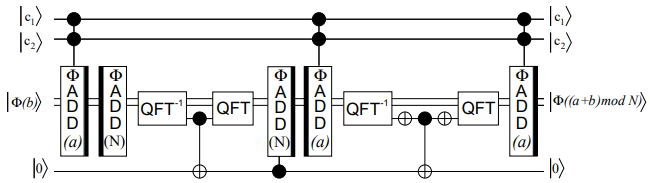
\includegraphics[width=\columnwidth]{Modular_adder_Paper.PNG}
  \centering
  \end{figure}
Abbildung~\ref{fig:modulare_addition_paper} zeigt das verwendete Konzept, 
das für die Implementierung der modularen Addition als Bauplan diente.
In der Grafik sind zwei Arten von \(\phi ADD\)-Gattern zu sehen.
Dabei handelt es sich um die Quanten-Addition, erkennbar mit dem fettgedruckten Strich auf der rechten Seite und 
der Quanten-Subtraktion mit einem fettgedruckten Strich auf der linken Seite.
Sowohl die Quanten-Addition als auch die Quanten-Subtraktion addieren beziehungsweise subtrahieren eine fixe Zahl und 
sind somit die zuvor vorgestellten Varianten mit gewöhnlichen Phasen-Gattern.
Der Quantenschaltkreis zur modularen Addition agiert als Baustein in einem größeren Gesamtbild, 
weshalb die zwei Kontroll-Qubits \(\ket{c_1}\) und \(\ket{c_2}\) eingebaut werden, 
die im weiteren Verlauf Anwendung finden.
Das Eingaberegister stellt auch das Zielregister dar und 
ist initial bereits in der Fourier-Basis mit \(\ket{\phi(b)}\).
Das Zielregister wird um ein weiteres Qubit erweitert, 
welches das Most-Significant-Bit des Zielregisters dargestellt.
Dieses Qubit hat einen besonderen Anwendungszweck und wird im weiteren als Borrow-Qubit bezeichnet.
Insgesamt besteht das Zielregister also aus \(n+1\) Qubits wenn der Modulus \(N\) einer Größenordnung von \(2^n\) entspricht.
Alle nachhaltigen Veränderungen durch den Quantenschaltkreis betreffen ausschließlich das Zielregister.
Des Weiteren verwendet die Quantenschaltung noch ein Qubit, welches initial im Zustand \(\ket{0}\) beginnt.
Der Zustand dieses einzelnen Qubits bedingt eine Fallunterscheidung in der Berechnung des Quantenschaltkreises und 
wird daher im Weiteren als Bedingungs-Qubit bezeichnet. 

Um die Berechnung des Quantenschaltkreises nachvollziehen zu können, 
wird die Auswirkung der verwendeten Gatter im einzelnen erklärt.
Die erste Quanten-Addition sorgt dafür, 
dass auf den initialen Zielregister \(\ket{\phi(b)}\) eine Addition mit \(a\) erfolgt und 
dadurch \(\ket{\phi(b + a)}\) entspricht.
Darauf folgt eine Quanten-Subtraktion die mit dem Subtrahend \(N\) auf das Zielregister mit
\(\ket{\phi(b + a - N)}\) wirkt. 
Daraus resultieren zwei mögliche Zustände:
\[1.~(b+a) \geq N~\rightarrow~\ket{\phi((b+a) - N)}_{n+1};~2.~
(b+a) < N~\rightarrow~\ket{\phi(2^{n+1}-(N-(a+b)))}_{n+1}
  \]
Im erste Fall entspricht das Ergebnis der korrekten Berechnung von \(a+b \mod N\).
In diesem Fall ist der Registerinhalt mit \(a+b \mod N\) kleiner als \(N\), 
weshalb das Borrow-Bit nicht gesetzt ist.
Im Gegensatz dazu ist das Ergebnis im zweiten Fall fehlerhaft.
Da bei \((b+a) < N\) bereits der Rest der modularen Restklasse im Register steht, 
wird durch die Quanten-Subtraktion ein \(N\) zu viel vom Registerinhalt abgezogen.
Dadurch entsteht ein underflow im Zielregister wodurch das Borrow-Bit gesetzt wird.

Als nächstes wirkt die inverse Quanten-Fourier-Transformation auf das Zielregister und führt eine Transformation in die Standartbasis durch.
Aufgrund des Basiswechsels in die Standartbasis beschreiben die Zustände der Qubits des Zielregisters nun das Ergebnis in der Binärdarstellung.
In der Binärdarstellung befindet sich im ersten Fall das Borrow-Bit im Zustand \(\ket{0}\) und im zweiten Fall im Zustand \(\ket{1}\).
Anhand dieser Unterscheidung kann man eine bedingte Operation mittels eines kontrollierten X-Gatter realisieren.
Dafür kontrolliert das Borrow-Bit ein X-Gatter welches auf das Bedingungs-Qubit wirkt.
Dadurch wird das Bedingungs-Qubit ausschließlich im zweiten Fall in den Zustand \(\ket{1}\) versetzt.
Danach wird das Zielregister wieder in die Fourier-Basis transformiert, 
indem die Quanten-Fourier-Transformation angewendet wird.
Anschließend kontrolliert das Bedingungs-Qubit eine Quanten-Addition mit dem Summanden \(N\) auf das Zielregister.
Die kontrollierte Quanten-Addition wird also nur im zweiten Fall angewendet und korrigiert das vorher ungültige Ergebnis,
zu dem korrekte:
\[
\ket{\phi(2^{n+1}-(N-(a+b)))}_{n+1} \underrightarrow{~+N~} 
\ket{\phi(2^{n+1}+(a+b))}_{n+1} \underrightarrow{\text{overflow }2^{n+1}}
\ket{\phi(a+b)}_{n+1}
  \]
Nun befinden sich in beiden Fällen das korrekt berechnete Ergebnis im Zielregister mit \(\ket{\Phi(a+b)\mod N}\).
Somit ist die Berechnung der modularen Addition abgeschlossen.

Je nach dem, welcher der beiden Fälle eingetreten ist, befindet sich das Bedingungs-Qubit in einem anderen Zustand.
Um zu verhindern, dass sich das Bedingungs-Qubit in einem ungewissen Zustand befindet und dadurch zum "`Trash"'-Qubit wird, 
wird der initiale Zustand \(\ket{0}\) des Bedingungs-Qubit durch die restlichen Gatter des Quantenschaltkreises wiederhergestellt.
Ein eindeutiger Zustand ermöglicht, dass das Bedingungs-Qubit bei weiteren Berechnungen wiederverwendet werden kann.

Um das Bedingungs-Qubit zurückzusetzen, 
wird zuerst eine Quanten-Subtraktion mit \(a\) auf das Zielregister angewendet.
Um die Auswirkungen dieser Quanten-Subtraktion hervorzuheben, wird der Registerinhalt für beide Fälle untersucht:
Im ersten Fall war \((b+a) \geq N\) weswegen die Subtraktion von \(N\) zum Ergebnis der modularen Addition führte.
Da \(a, b < N\) gilt, ist das Ergebnis der modularen Addition kleiner als \(a\).
Die Quanten-Subtraktion mit \(a\) führt also zu einem Underflow, wodurch das Borrow-Bit gesetzt wird.
Im zweiten Fall, war \((b+a) < N\).
Deswegen wurde die Subtraktion von \(N\) nicht durchgeführt, 
beziehungsweise wieder rückgängig gemacht, da \((b+a)\) bereits das Ergebnis der modularen Addition ist.
Für den zweiten Fall gilt als Ergebnis also \((b+a)\) und dies ist größer als \(a\), 
darum kommt es zu keinem Underflow und das Borrow-Bit ist deswegen nicht gesetzt.
Der Zustand des Borrow-Bits ist nun also im Vergleich zu den Fällen des vorherigen Abschnitts der Quantenschaltung invertiert.

Um das Borrow-Bit auslesen zu können, 
wird analog zum vorherigen Abschnitt des Quantenschaltkreises eine inverse Quanten-Fourier-Transformation durchgeführt.
Anschließend wird ein X-Gatter auf das Borrow-Bit angewendet.
Dadurch befindet sich das Borrow-Bit nun in denselben Zuständen wie in den beiden Fällen des ersten Abschnitts der Quantenschaltung.
Im nächsten Schritt kontrolliert das Borrow-Bit ein X-Gatter, das auf das Bedingungs-Qubit wirkt.
Dadurch wird es wieder in den initialen Zustand \(\ket{0}\) versetzt.

Um den Zustand \(\ket{\Phi(a+b)\mod N}\) des Zielregister wiederherzustellen, 
werden die Gatter bis zur Quanten-Subtraktion mit \(a\) inverse angewendet.
Zunächst wird ein selbstinverses X-Gatter auf das Borrow-Bit angewendet.
Danach folgt die Quanten-Fourier-Transformation, 
die die Inverse der inversen Quanten-Fourier-Transformation darstellt.
Abschließend folgt die Quanten-Addition mit \(a\), 
um die zuvor erfolgte Quanten-Subtraktion von \(a\) auf das Zielregister zu revertieren.

Das Zielregisters beinhaltet nun also den gewünschten Zustand \(\ket{\Phi(a+b)\mod N}\) für \(a, b < N\).
Des weiteren befindet sich das Bedingungs-Qubit wieder im initialen Zustand und kann für weitere Rechnungen wiederverwendet werden.

\vspace{1em}

Wenn man den Quantenschaltkreis in Abbildung~\ref{fig:modulare_addition_paper} betrachtet,
fällt auf, fällt auf, 
dass nicht alle Quanten-Additionen und Quanten-Subtraktionen kontrolliert durchgeführt werden.
Die modulare Addition soll nur dann ausgeführt werden, wenn die Kontroll-Qubits \(\ket{c_1}\) und \(\ket{c_2}\) gesetzt sind.
Dies ist zurückzuführen auf die Bedingung \(b < N\), 
die dafür sorgt, dass der Rest des Quantenschaltkreises lediglich die Identitätstransformation durchführt, 
wenn die Kontroll-Qubits nicht aktiviert sind~\cite{beauregard2003circuit}.
Der Grund, weshalb nicht alle Quanten-Additionen, 
Quanten-Subtraktion und gegebenenfalls sogar die (inversen) Quanten-Fourier-Transformationen kontrolliert sind,
liegt in der erhöhten Komplexität, die dadurch im Quantenschaltkreis entstehen würde~\cite{beauregard2003circuit}.
Wenn ein Kontroll-Qubit nicht aktiviert ist, wird das kontrollierte Gatter zwar ausgeführt, jedoch ohne praktische Wirkung.
Abbildung~\ref{fig:gatedef_U1U2U3_CNOT} zeigt die physikalische Implementierung dreier Single-Qubit-Gatter im Vergleich zu einem kontrollierten X-Gatter.
Wie aus der Abbildung erkennbar, 
benötigt das kontrollierte Gatter mehr Hardware-Elemente als die drei Single-Qubit-Gatter.
Somit ist es nicht möglich die Komplexität des Quantenschaltkreis zu verringern, 
indem zusätzliche Gatter kontrolliert angewendet werden.
\begin{figure} [H]
  \caption{Physikalische Implementierung~\cite{ibmqx5}}
  \label{fig:gatedef_U1U2U3_CNOT}
  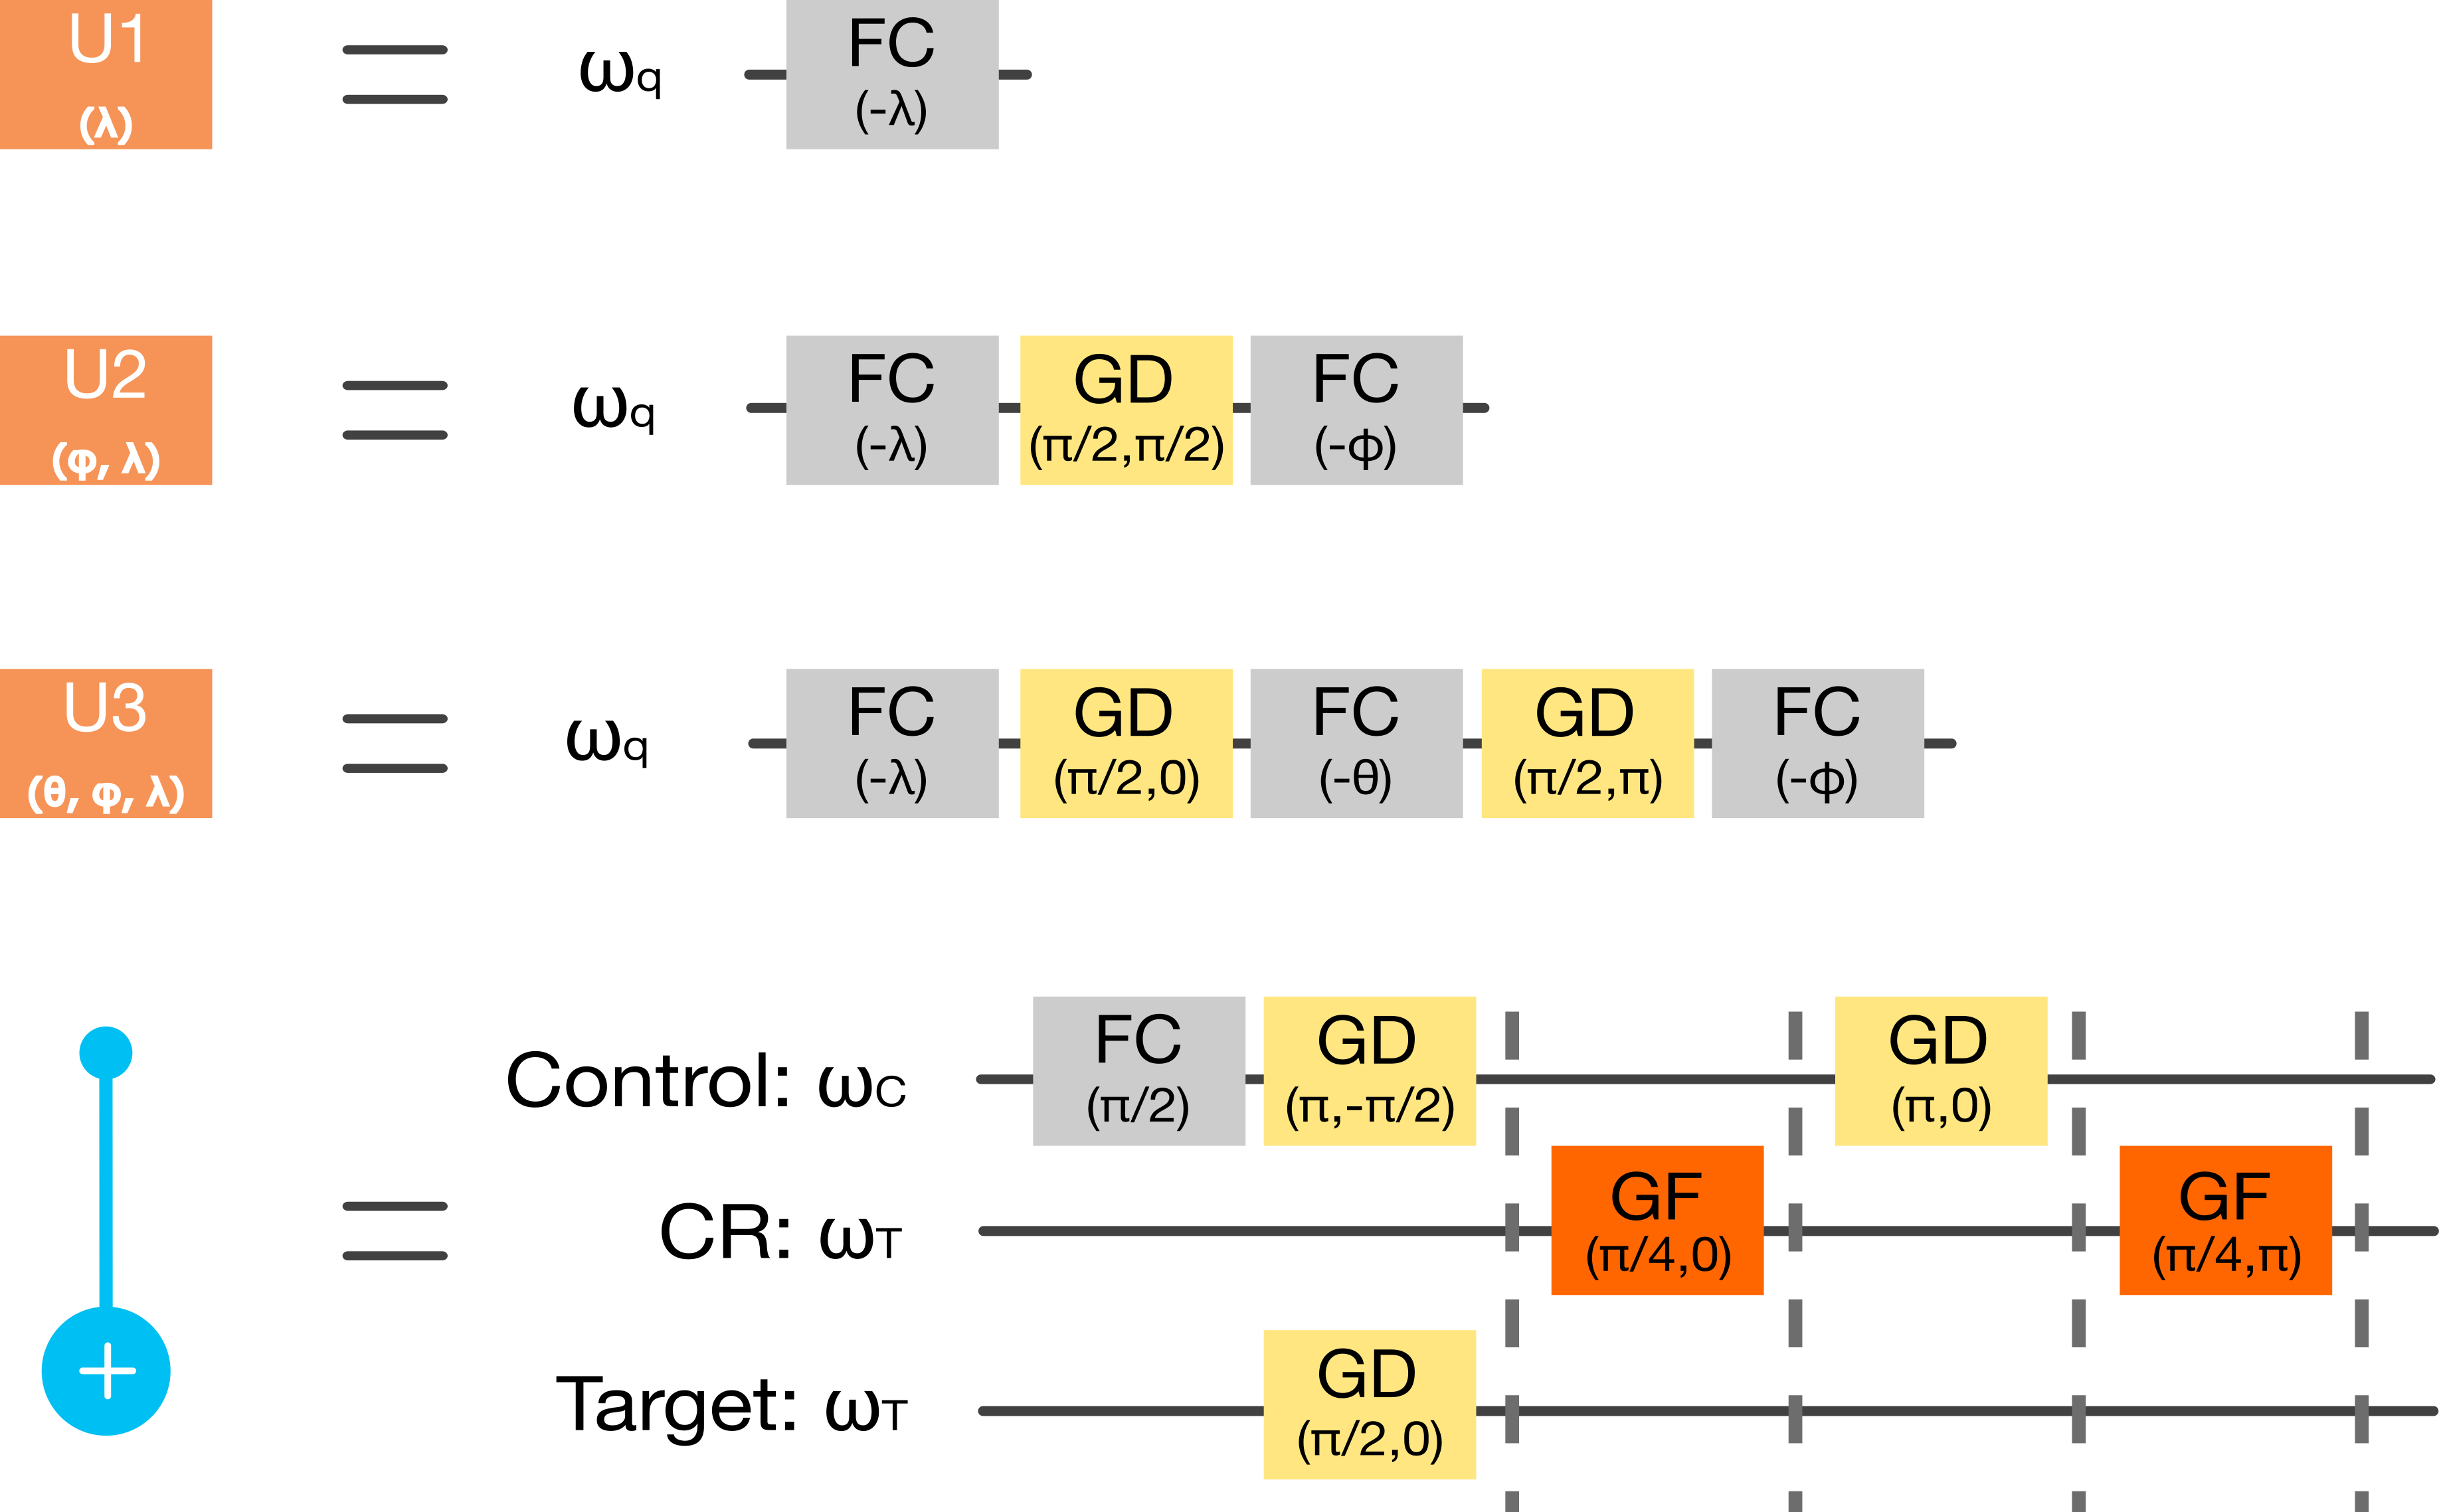
\includegraphics[width=\columnwidth,height=10cm]{gatedef_U1U2U3_CNOT.png}
  \centering
  \end{figure}

Ein weiterer Aspekt, 
der die Komplexität der Quantenschaltung für die modulare Addition erhöht, 
ist der Abschnitt, der das Bedingungs-Qubit zurücksetzt.
Wäre es möglich, diesen Teil auszulassen, könnten zwei der insgesamt fünf Quanten-Additionen bzw. 
Quanten-Subtraktionen sowie die Hälfte der (inversen) Quanten-Fourier-Transformationen eingespart werden.

Es gibt die Möglichkeit, bei einem Qubit einen Reset durchzuführen, wodurch dieses den Zustand \(\ket{0}\) annimmt.
In Qiskit kann dies mit der Funktion \texttt(Reset)~\cite{qiskitReset} realisiert werden.
Die Verwendung ist jedoch nicht zielführend, da diese durch keine unitäre Abbildungsmatrix
beschrieben werden kann.
Somit ist die Reset Transformation nicht unitär und würde deswegen dazu führen, dass alle Quantenalgorithmen, 
die diese Funktion nutzen, ebenfalls nicht mehr unitär wären.
Da die Quanten-Phase-Estimation den Eigenwert einer unitären Transformation extrahiert, 
ist diese Funktion für die Anwendung im Shor-Algorithmus ungeeignet.

\begin{figure} [H]
  \caption{Qiskit modulare Addition}
  \label{fig:ModularAddition}
  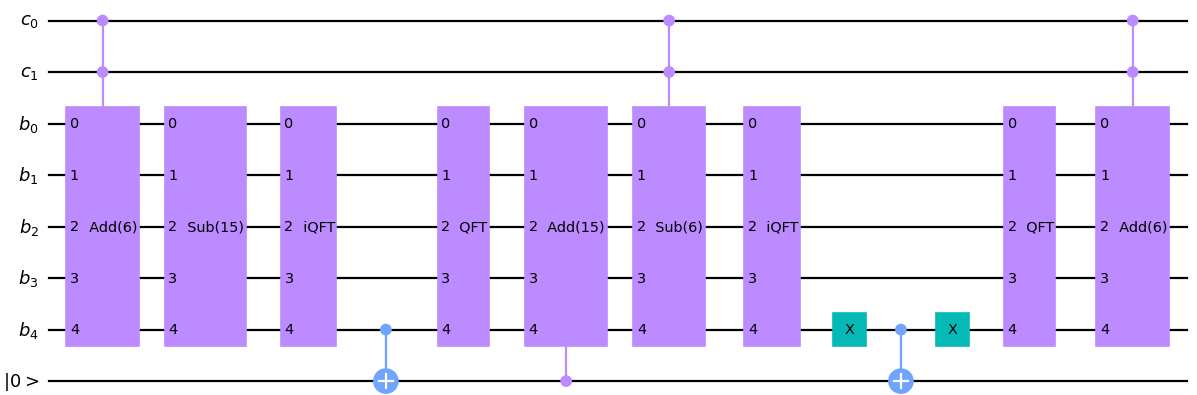
\includegraphics[width=\columnwidth]{modulareAddition.png}
  \centering
  \end{figure}

Abbildung~\ref{fig:ModularAddition} zeigt die Implementierung in Qiskit, 
die durch den Code der Funktion \texttt{Modular\_Adder\_Gate}~\ref{code:ModularAddition} beschrieben wird.
Die Funktion \texttt{Modular\_Adder\_Gate} erwartet als Parameter den Summand \(a\) und die Zahl \(N\) jeweils als eine 
Liste, welche die Zahl in Binärdarstellung beschreibt.
Dabei repräsentiert der erste Index beider Listen das Least-Significant-Bit.
Wenn \(N\) der Größenordnung \(2^n\) entspricht, 
müssen die Listen jeweils von der Länge \(n+1\) sein wobei das Most-Significant-Bit der \(0\) entspricht.
Die Funktion definiert drei Wertebereiche, die die Positionen der Qubits beschreiben.
\textit{c\_qbits} definiert die beiden Kontroll-Qubits, \textit{b\_qbits} die Qubits, welche den Summanden  \(b\) 
in der Fourier-Basis enthalten und textit{cond\_qbit} repräsentiert die Position des Bedingungs-Qubit.
Dadurch das \textit{b\_qbits} genau so groß definiert wird, 
wie die Liste des Summand \(a\) lang ist, wird sichergestellt, 
dass das \textit{b\_qbits} Register ein extra Qubit enthält für das Borrow-Bit.


 

\begin{figure}[H]
  \caption{Modulare Addition in Qiskit}
  \label{code:ModularAddition}
\begin{minted}[linenos]{python}    
def Modular_Adder_Gate(a_bin: list[int],N_bin: list[int]) -> qiskit.circuit.gate:
  c_qbits = [0,1]
  b_qbits = list(range(2, len(a_bin)+2))
  cond_qbit = len(a_bin)+2
  m_a_g = qiskit.QuantumCircuit(2 + len(a_bin) + 1) 
  m_a_g.append(A_Gate(a_bin).control(2), c_qbits + b_qbits)
  m_a_g.append(S_Gate(N_bin),b_qbits)
  m_a_g.append(QFT_Gate(len(a_bin),inverse = True, MSB_first = False), b_qbits)
  m_a_g.cnot(b_qbits[-1],cond_qbit)
  m_a_g.append(QFT_Gate(len(a_bin),inverse = False, MSB_first = False), b_qbits)
  m_a_g.append(A_Gate(N_bin).control(1), [cond_qbit] + b_qbits)
  m_a_g.append(S_Gate(a_bin).control(2), c_qbits + b_qbits)
  m_a_g.append(QFT_Gate(len(a_bin),inverse = True, MSB_first = False), b_qbits)
  m_a_g.x(b_qbits[-1])
  m_a_g.cnot(b_qbits[-1],cond_qbit)
  m_a_g.x(b_qbits[-1])
  m_a_g.append(QFT_Gate(len(a_bin),inverse = False, MSB_first = False), b_qbits)
  m_a_g.append(A_Gate(a_bin).control(2), c_qbits + b_qbits)
  m_a_g = m_a_g.to_gate()
  m_a_g.name = "Add " + str(binToDez(a_bin)) + " Mod " + str(binToDez(N_bin))
  return m_a_g
  \end{minted}
\end{figure}




















